\documentclass[10pt]{beamer}\usepackage[]{graphicx}\usepackage[]{color}
%% maxwidth is the original width if it is less than linewidth
%% otherwise use linewidth (to make sure the graphics do not exceed the margin)
\makeatletter
\def\maxwidth{ %
  \ifdim\Gin@nat@width>\linewidth
    \linewidth
  \else
    \Gin@nat@width
  \fi
}
\makeatother

\definecolor{fgcolor}{rgb}{0.345, 0.345, 0.345}
\newcommand{\hlnum}[1]{\textcolor[rgb]{0.686,0.059,0.569}{#1}}%
\newcommand{\hlstr}[1]{\textcolor[rgb]{0.192,0.494,0.8}{#1}}%
\newcommand{\hlcom}[1]{\textcolor[rgb]{0.678,0.584,0.686}{\textit{#1}}}%
\newcommand{\hlopt}[1]{\textcolor[rgb]{0,0,0}{#1}}%
\newcommand{\hlstd}[1]{\textcolor[rgb]{0.345,0.345,0.345}{#1}}%
\newcommand{\hlkwa}[1]{\textcolor[rgb]{0.161,0.373,0.58}{\textbf{#1}}}%
\newcommand{\hlkwb}[1]{\textcolor[rgb]{0.69,0.353,0.396}{#1}}%
\newcommand{\hlkwc}[1]{\textcolor[rgb]{0.333,0.667,0.333}{#1}}%
\newcommand{\hlkwd}[1]{\textcolor[rgb]{0.737,0.353,0.396}{\textbf{#1}}}%
\let\hlipl\hlkwb

\usepackage{framed}
\makeatletter
\newenvironment{kframe}{%
 \def\at@end@of@kframe{}%
 \ifinner\ifhmode%
  \def\at@end@of@kframe{\end{minipage}}%
  \begin{minipage}{\columnwidth}%
 \fi\fi%
 \def\FrameCommand##1{\hskip\@totalleftmargin \hskip-\fboxsep
 \colorbox{shadecolor}{##1}\hskip-\fboxsep
     % There is no \\@totalrightmargin, so:
     \hskip-\linewidth \hskip-\@totalleftmargin \hskip\columnwidth}%
 \MakeFramed {\advance\hsize-\width
   \@totalleftmargin\z@ \linewidth\hsize
   \@setminipage}}%
 {\par\unskip\endMakeFramed%
 \at@end@of@kframe}
\makeatother

\definecolor{shadecolor}{rgb}{.97, .97, .97}
\definecolor{messagecolor}{rgb}{0, 0, 0}
\definecolor{warningcolor}{rgb}{1, 0, 1}
\definecolor{errorcolor}{rgb}{1, 0, 0}
\newenvironment{knitrout}{}{} % an empty environment to be redefined in TeX

\usepackage{alltt}%
\usetheme{Boadilla}
\usecolortheme{seahorse}

\usepackage[utf8]{inputenc}%

% graphics
%% Figures %%%%%%%%%%%%%%%%%%%%%%%%%%%%%%%%%%%%%%%%%%%%%%%%%%
\usepackage{graphicx}
\usepackage{xcolor}%for color mixing

\usepackage{amsmath}%
\usepackage{amsfonts}%
\usepackage{amssymb}%
\usepackage{graphicx}

\usepackage{tikz}

%%%%%%%%%%%%%%%%%%%%%%%%%%%%%%%%%%%%%%%%%%%%%%
%%%%%%%%%%%%%%%%% Doc info %%%%%%%%%%%%%%%%%%%
\title[\textbf{Linear models 2:}]{What on earth is going on with my linear models??!}
\date{\today}

%%%%%%%%%%%%%%%%%%%%%%%%%%%%%%%%%%%%
\IfFileExists{upquote.sty}{\usepackage{upquote}}{}
\begin{document}




\begin{frame}
\maketitle	
\end{frame}
%%%%%%%%%%%

\AtBeginSection[]
{
  \begin{frame}<beamer>
    \frametitle{}
    \tableofcontents[currentsection,hideothersubsections,subsectionstyle=hide]% down vote\tableofcontents[currentsection,currentsubsection,hideothersubsections,sectionstyle=show/hide,subsectionstyle=show/shaded/hide] 
  \end{frame}
} 



%%%%%%%%%%%%%%%%%%%%%%%%%%%%%%%%%%%%%%%%%%%%%%%%%%%%%%%%%%%%%%%%%%%
%%%%%%%%%%%%%%%%%%%%%%%%%%%%%%%%%%%%%%%%%%%%%%%%%%%%%%%%%%%%%%%%%%%
\section{Linear model, reminder}

\begin{frame}[fragile]{A simple linear model}
  \textbf{{\color{purple}{Response}} = {\color{blue}{Intercept}} + {\color{red}{Slope}} $\times$ {\color{orange}{Predictor}} + {\color{gray}{Error}}} \\
  
\begin{knitrout}\small
\definecolor{shadecolor}{rgb}{0.843, 0.867, 0.922}\color{fgcolor}
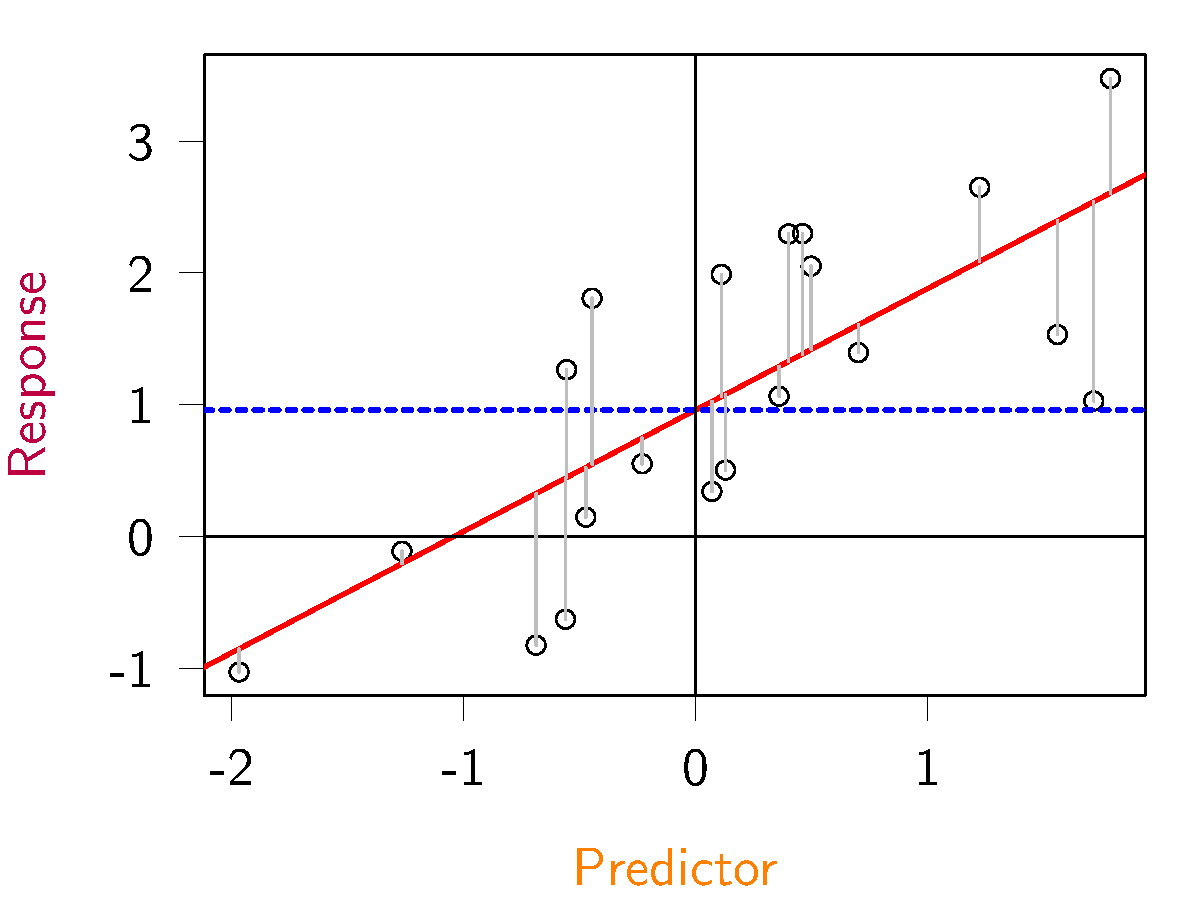
\includegraphics[width=0.8\textwidth,height=0.6\textwidth]{figure/lmprinc-1} 

\end{knitrout}
\end{frame}
%%%%%%%%%%%

\begin{frame}[fragile]{A simple linear model}
  \textbf{{\color{purple}{Response}} = {\color{blue}{Intercept}} + {\color{red}{Slope}} $\times$ {\color{orange}{Predictor}} + {\color{gray}{Error}}} \\
  \vspace{1cm}
\textbf{In R:}
\begin{knitrout}\small
\definecolor{shadecolor}{rgb}{0.843, 0.867, 0.922}\color{fgcolor}\begin{kframe}
\begin{alltt}
  \hlkwd{lm}\hlstd{(response} \hlopt{~} \hlnum{1} \hlopt{+} \hlstd{predictor1} \hlopt{+} \hlstd{predictor2,} \hlkwc{data}\hlstd{=data)}
\end{alltt}
\end{kframe}
\end{knitrout}
\begin{itemize}
  \item Intercept can be explicit or implicit
  \item Can remove intercept with \texttt{\dots $\sim $ 0 + \dots}
  \item Error is implicit
  \item Feed the option \texttt{data=} to keep code short, reliable and flexible
  \item Order of predictors do not matter 
\end{itemize}

\end{frame}
%%%%%%%%%%%

%%%%%%%%%%%%%%%%%%%%%%%%%%%%%%%%%%%%%%%%%%%%%%%%%%%%%%%%%%%%%%%%%%%%%%%%%%%%%%%%%%%%%%%%%%%%%%%%%%%%
\section{Diagnostics}

\begin{frame}[fragile]{Why we need checks: summary(lm) isn't enough}

\begin{knitrout}\small
\definecolor{shadecolor}{rgb}{0.843, 0.867, 0.922}\color{fgcolor}\begin{kframe}
\begin{alltt}
  \hlstd{Ans} \hlkwb{<-} \hlkwd{read.csv}\hlstd{(}\hlkwc{file} \hlstd{=} \hlstr{"Anscombe.csv"}\hlstd{)}
\end{alltt}
\end{kframe}
\end{knitrout}
  
\begin{knitrout}\small
\definecolor{shadecolor}{rgb}{0.843, 0.867, 0.922}\color{fgcolor}
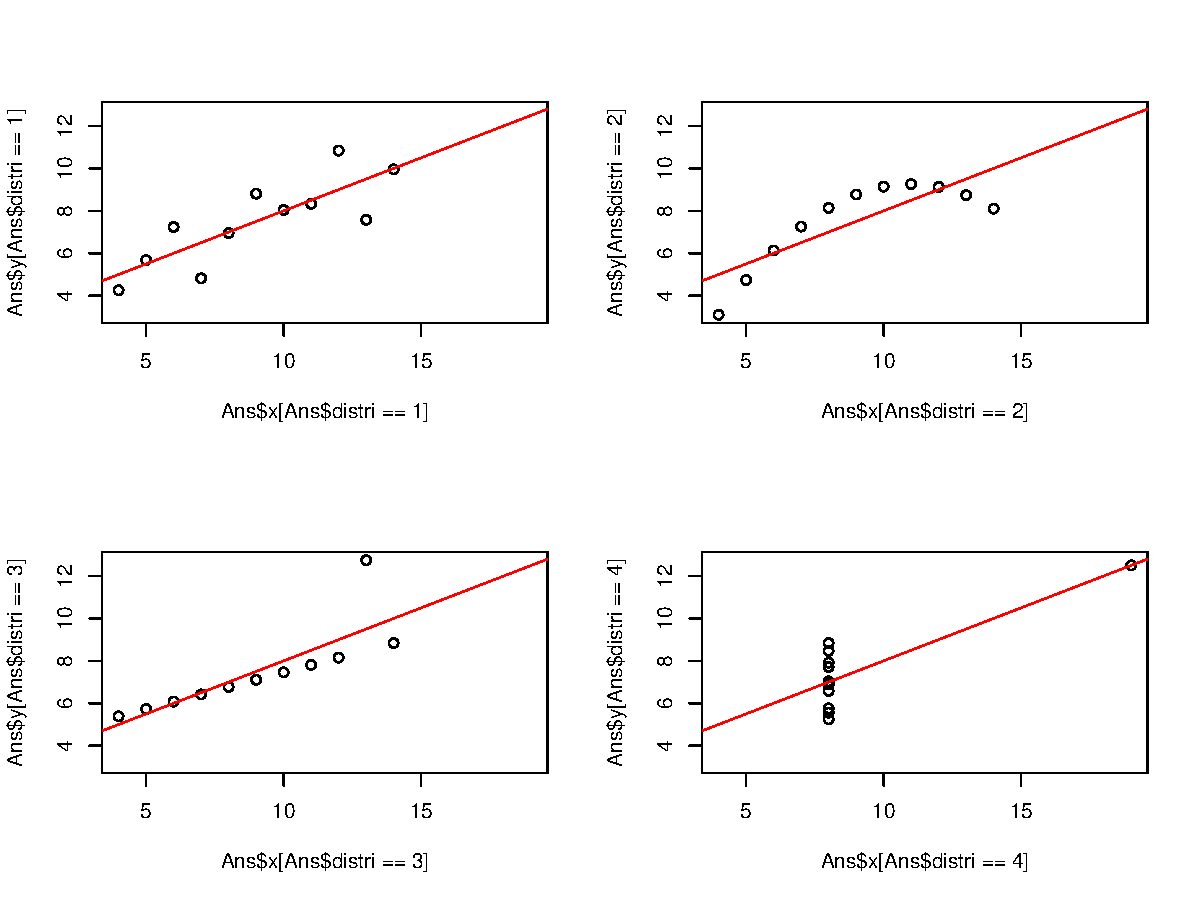
\includegraphics[width=0.8\textwidth,height=0.6\textwidth]{figure/anscombe-1} 

\end{knitrout}
\end{frame}
%%%%%%%%%%%

\begin{frame}{General approach}

\begin{center}
  \begin{tikzpicture}
    \node (sq) at (0,-1) {\color{red}{1. Scientific question}};
    \node (mo) at (0,-2) {2. Model and Statistical question};
    \draw[->, thick] (sq)--(mo);
    \node (dac) at (6,-2) {\color{red}{3. Data collection}};
    \draw[<->, thick] (mo)--(dac);

    \node (est) at (0,-3) {4. Estimation};
        \draw[->, thick] (mo)--(est);
    \node (unc) at (0,-3.5) {4.b Uncertainty and statistical significance};
    
    \node (che) at (0,-5) {\textbf{5. Diagnostic, check assumptions, prediction}};
        \draw[->, thick] (unc)--(che);
    \draw[->, thick] (che.west) to [out=150, in=210] (mo.west);

    \node (int) at (0,-6) {\color{red}{6. Interpret and think about the biology}};
        \draw[->, thick] (che)--(int);

  \draw[rounded corners, color=blue] (-4.5,-1.5) rectangle (4,-5.5);
  \node[anchor=north west] (r) at (-4.5,-1.5) {
\includegraphics[width=0.1\textwidth]{Figures/r}};
  \end{tikzpicture}
  \end{center}
\end{frame}
%%%%%%%%%%%

%%%%%%%%%%%%%%%%%%%%%%%%%%%%%%%%%%%%%%%%%%%%%%%%%%%%%%%%%%%%%%%%%%%%%%%%%%%%%%%%%%%%%%%%
\begin{frame}{Linear model basic assumptions}
Not necessarily wrong, but typical interpretation assumes:
 \begin{block}{}
     \begin{itemize}[<+->]
      \item Linear combination of parameters (including transformation, polynoms, interactions\dots)\\ \textit{Risk: biologically meaningless; e.g. static allometry}
      \item Predictor not perfectly correlated \\ \textit{Risk: Model won't run, unstable convergence, or huge SE}
       \item {\color{red!20!black}{Measurement error in predictors}}\\ \textit{Risk: bias estimates (underestimate with Gaussian error)}
       \item {\color{red!50!black}{Gaussian error distribution}}\\ \textit{Risk: Poor predictions}
       \item {\color{red!70!black}{Homoscedasticity (constant error variance)}}\\ \textit{Risk: Over-optimistic uncertainty, unreliable predictions}
       \item {\color{red!99!black}{Independence of error}}\\ \textit{Risk: Bias and over-optimistic uncertainty}
     \end{itemize}
 \end{block}
\end{frame}
%%%%%%%%%%%

\begin{frame}[fragile]{Why we need checks: missing a relationship}
  


\begin{knitrout}\small
\definecolor{shadecolor}{rgb}{0.843, 0.867, 0.922}\color{fgcolor}\begin{kframe}
\begin{alltt}
 \hlstd{forprediction} \hlkwb{<-} \hlkwd{read.csv}\hlstd{(}\hlkwc{file} \hlstd{=} \hlstr{"forprediction.csv"}\hlstd{)}
\end{alltt}
\end{kframe}
\end{knitrout}
  Does "predictor" predict "obs"? 
 \pause

\begin{knitrout}\small
\definecolor{shadecolor}{rgb}{0.843, 0.867, 0.922}\color{fgcolor}\begin{kframe}
\begin{alltt}
  \hlkwd{summary}\hlstd{(}\hlkwd{lm}\hlstd{(obs} \hlopt{~} \hlnum{1} \hlopt{+} \hlstd{predictor,} \hlkwc{data}\hlstd{=forprediction) )}
\end{alltt}
\end{kframe}
\end{knitrout}
\end{frame}
%%%%%%%%%%%

\begin{frame}[fragile]{Why we need checks: missing a relationship}
  Does "predictor" predict "obs"? Apparently not:
\begin{knitrout}\small
\definecolor{shadecolor}{rgb}{0.843, 0.867, 0.922}\color{fgcolor}\begin{kframe}
\begin{alltt}
  \hlkwd{summary}\hlstd{(}\hlkwd{lm}\hlstd{(obs} \hlopt{~} \hlnum{1} \hlopt{+} \hlstd{predictor,} \hlkwc{data}\hlstd{=forprediction) )}
\end{alltt}
\begin{verbatim}

Call:
lm(formula = obs ~ 1 + predictor, data = forprediction)

Residuals:
    Min      1Q  Median      3Q     Max 
-2.1962 -0.5326  0.1378  0.5785  1.8664 

Coefficients:
            Estimate Std. Error t value Pr(>|t|)    
(Intercept)  2.72530    0.16953  16.076   <2e-16 ***
predictor   -0.01129    0.02956  -0.382    0.703    
---
Signif. codes:  0 '***' 0.001 '**' 0.01 '*' 0.05 '.' 0.1 ' ' 1

Residual standard error: 0.8382 on 98 degrees of freedom
Multiple R-squared:  0.001487,	Adjusted R-squared:  -0.008702 
F-statistic: 0.1459 on 1 and 98 DF,  p-value: 0.7033
\end{verbatim}
\end{kframe}
\end{knitrout}
\end{frame}
%%%%%%%%%%%

\begin{frame}[fragile]{Why we need checks: missing a relationship}

\begin{knitrout}\small
\definecolor{shadecolor}{rgb}{0.843, 0.867, 0.922}\color{fgcolor}
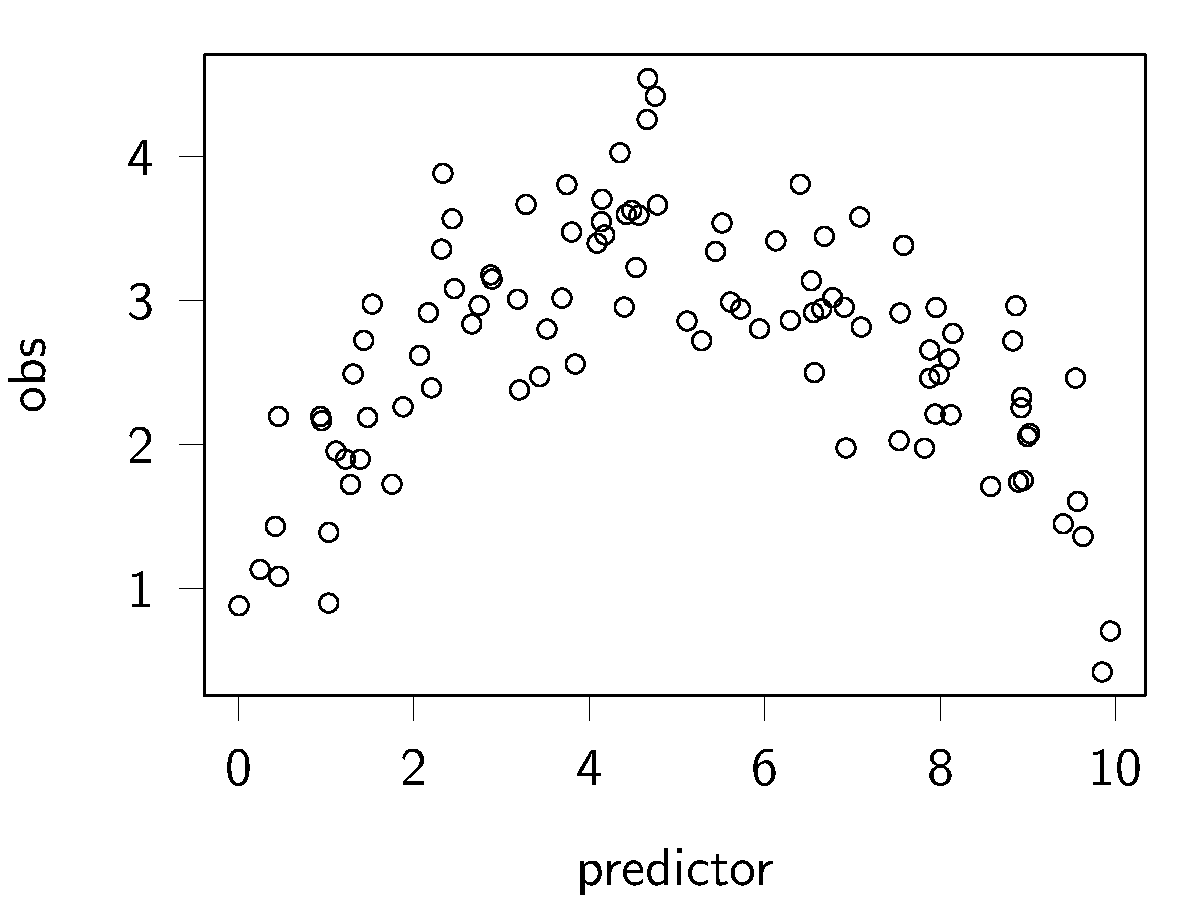
\includegraphics[width=0.8\textwidth,height=0.6\textwidth]{figure/plot0-1} 

\end{knitrout}

\end{frame}
%%%%%%%%%%%

\begin{frame}[fragile]{How to check?}
\begin{knitrout}\small
\definecolor{shadecolor}{rgb}{0.843, 0.867, 0.922}\color{fgcolor}\begin{kframe}
\begin{alltt}
\hlstd{m0} \hlkwb{<-} \hlkwd{lm}\hlstd{(obs} \hlopt{~} \hlnum{1} \hlopt{+} \hlstd{predictor,} \hlkwc{data}\hlstd{=forprediction)}
\hlkwd{summary}\hlstd{(m0)}
\end{alltt}
\begin{verbatim}

Call:
lm(formula = obs ~ 1 + predictor, data = forprediction)

Residuals:
    Min      1Q  Median      3Q     Max 
-2.1962 -0.5326  0.1378  0.5785  1.8664 

Coefficients:
            Estimate Std. Error t value Pr(>|t|)    
(Intercept)  2.72530    0.16953  16.076   <2e-16 ***
predictor   -0.01129    0.02956  -0.382    0.703    
---
Signif. codes:  0 '***' 0.001 '**' 0.01 '*' 0.05 '.' 0.1 ' ' 1

Residual standard error: 0.8382 on 98 degrees of freedom
Multiple R-squared:  0.001487,	Adjusted R-squared:  -0.008702 
F-statistic: 0.1459 on 1 and 98 DF,  p-value: 0.7033
\end{verbatim}
\end{kframe}
\end{knitrout}
\end{frame}
%%%%%%%%%%%


\begin{frame}[fragile]{How to check?}
\begin{knitrout}\small
\definecolor{shadecolor}{rgb}{0.843, 0.867, 0.922}\color{fgcolor}\begin{kframe}
\begin{alltt}
\hlkwd{par}\hlstd{(}\hlkwc{mfrow}\hlstd{=}\hlkwd{c}\hlstd{(}\hlnum{2}\hlstd{,}\hlnum{2}\hlstd{))}
  \hlkwd{plot}\hlstd{(m0)}
\end{alltt}
\end{kframe}
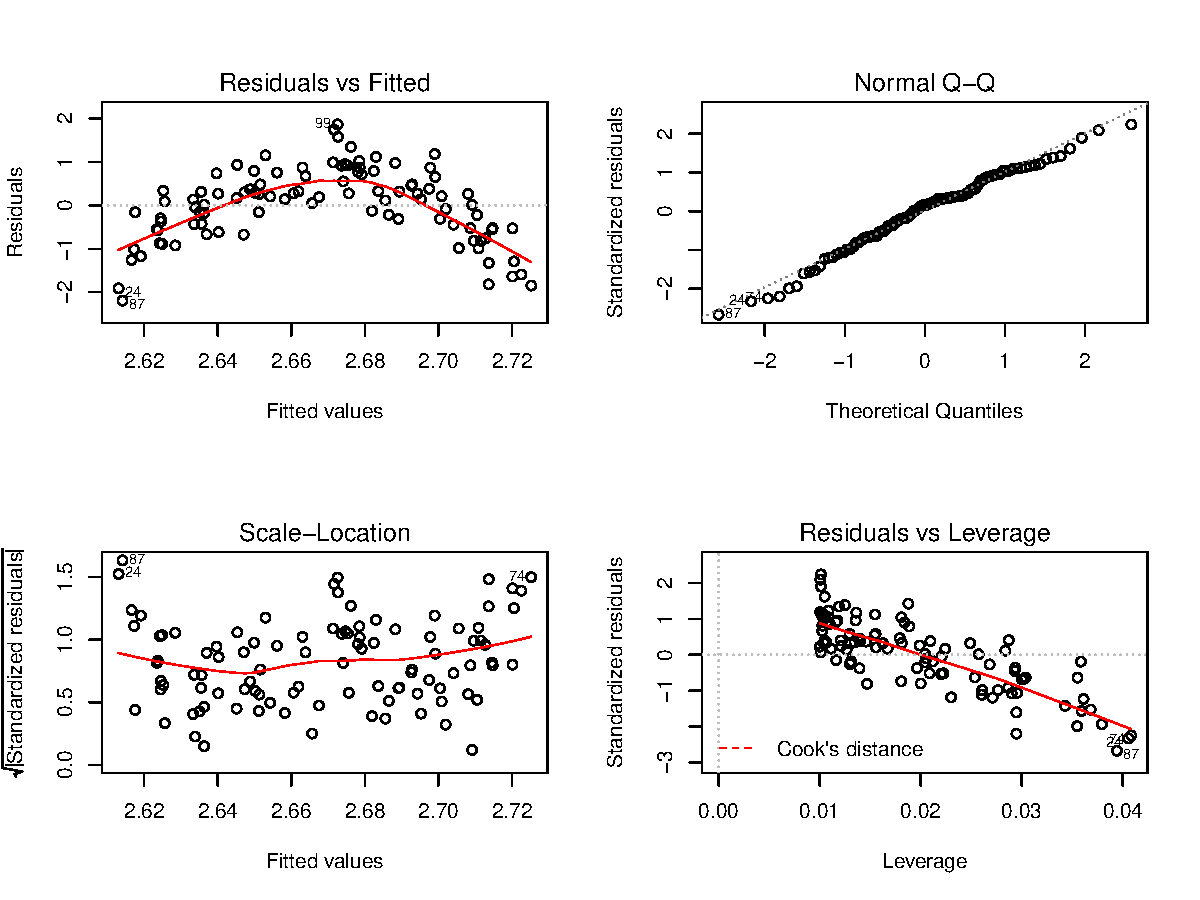
\includegraphics[width=0.8\textwidth,height=0.6\textwidth]{figure/unnamed-chunk-8-1} 
\begin{kframe}\begin{alltt}
\hlkwd{par}\hlstd{(}\hlkwc{mfrow}\hlstd{=}\hlkwd{c}\hlstd{(}\hlnum{1}\hlstd{,}\hlnum{1}\hlstd{))}
\end{alltt}
\end{kframe}
\end{knitrout}
\end{frame}
%%%%%%%%%%%

\begin{frame}[fragile]{How to check?}

\begin{knitrout}\small
\definecolor{shadecolor}{rgb}{0.843, 0.867, 0.922}\color{fgcolor}\begin{kframe}
\begin{alltt}
\hlstd{m0} \hlkwb{<-} \hlkwd{lm}\hlstd{(obs} \hlopt{~} \hlnum{1} \hlopt{+} \hlstd{predictor,} \hlkwc{data}\hlstd{=forprediction)}
\end{alltt}
\end{kframe}
\end{knitrout}
    \centering
\begin{knitrout}\small
\definecolor{shadecolor}{rgb}{0.843, 0.867, 0.922}\color{fgcolor}\begin{kframe}
\begin{alltt}
    \hlkwd{setPar}\hlstd{()}
\hlkwd{plot}\hlstd{(}\hlkwc{x}\hlstd{=forprediction}\hlopt{$}\hlstd{predictor,} \hlkwc{y}\hlstd{=forprediction}\hlopt{$}\hlstd{obs,} \hlkwc{xlab}\hlstd{=}\hlstr{"predictor"}\hlstd{,} \hlkwc{ylab}\hlstd{=}\hlstr{"obs"}\hlstd{)}
\hlkwd{abline}\hlstd{(m0,} \hlkwc{col}\hlstd{=}\hlstr{"red"}\hlstd{,} \hlkwc{lwd}\hlstd{=}\hlnum{3}\hlstd{)} \hlcom{#simple prediction, without SE}
\end{alltt}
\end{kframe}
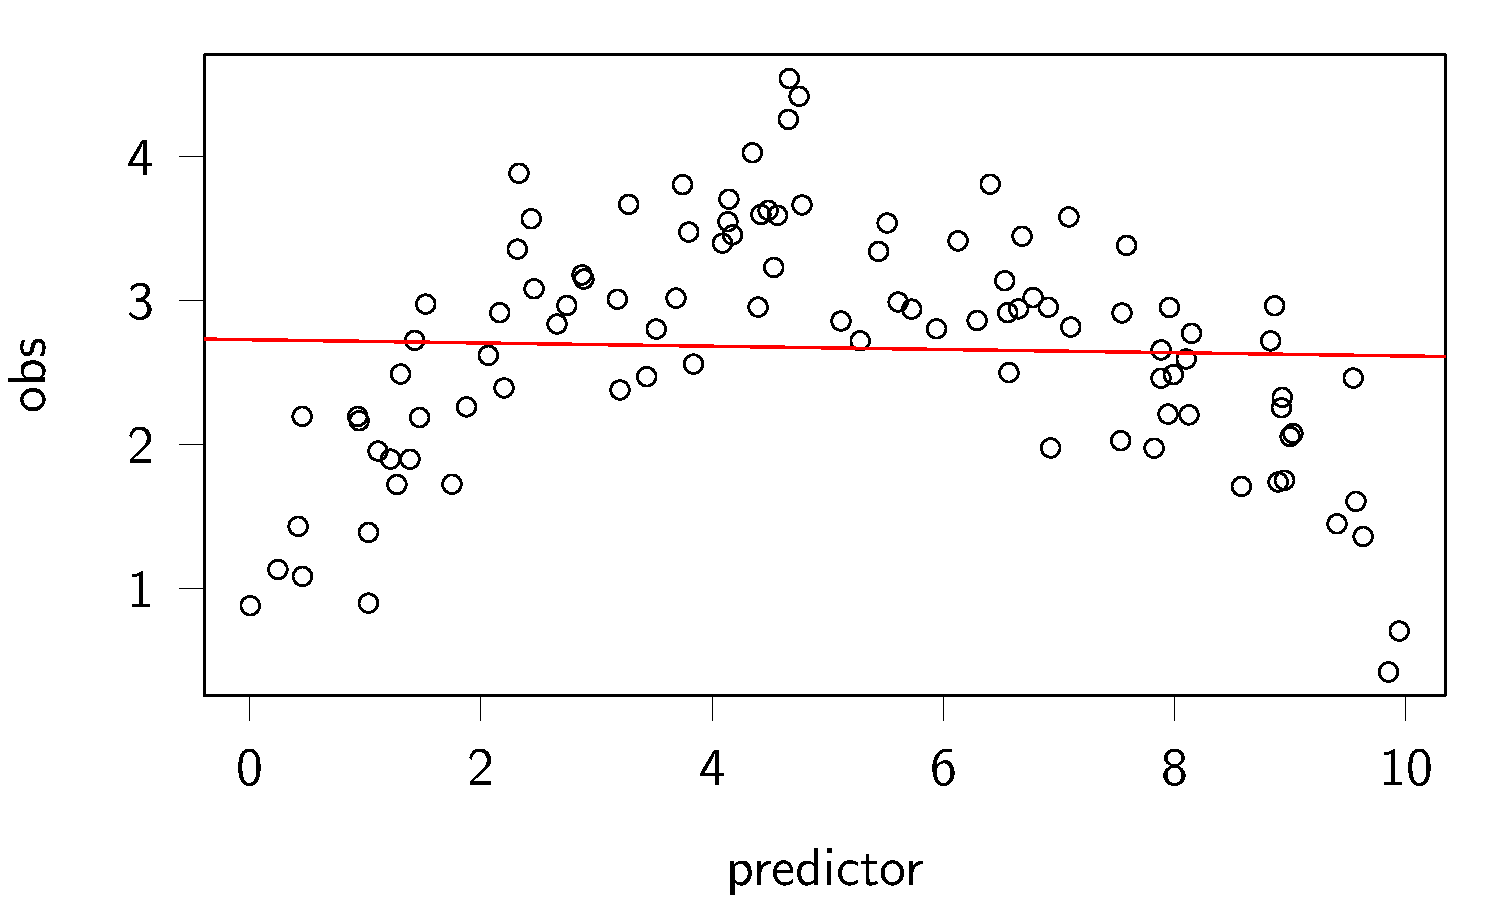
\includegraphics[width=0.8\textwidth,height=0.6\textheight]{figure/plot0plusabline-1} 

\end{knitrout}

\end{frame}
%%%%%%%%%%%

\begin{frame}{Check checklist}
  \begin{exampleblock}{}
    \begin{itemize}
      \item \textbf{Visualize your data}
      \item Residual in summary(): are they symmetrical?
      \item plot(lm):
        \begin{enumerate}
          \item trend residual/fitted?
          \item Normal residuals?
          \item trend in residual variance?
          \item outliers?
        \end{enumerate}
      \item Predictions: range and biological meaning
    \end{itemize}
  \end{exampleblock}
  
  
\end{frame}
%%%%%%%%%%

\begin{frame}[fragile]{Fix?}

Plot suggests a quadratic relationship

\begin{knitrout}\small
\definecolor{shadecolor}{rgb}{0.843, 0.867, 0.922}\color{fgcolor}\begin{kframe}
\begin{alltt}
\hlkwd{lm}\hlstd{(obs} \hlopt{~} \hlnum{1} \hlopt{+} \hlstd{predictor ,} \hlkwc{data}\hlstd{=forprediction)}
\end{alltt}
\end{kframe}
\end{knitrout}
  \pause

\begin{knitrout}\small
\definecolor{shadecolor}{rgb}{0.843, 0.867, 0.922}\color{fgcolor}\begin{kframe}
\begin{alltt}
\hlstd{m1} \hlkwb{<-} \hlkwd{lm}\hlstd{(obs} \hlopt{~} \hlnum{1} \hlopt{+} \hlstd{predictor} \hlopt{+} \hlkwd{I}\hlstd{(predictor}\hlopt{^}\hlnum{2}\hlstd{),} \hlkwc{data}\hlstd{=forprediction)}
\hlkwd{plot}\hlstd{(m1)}
\end{alltt}
\end{kframe}
\end{knitrout}

  How about prediction? (abline(m1) won't work here because not straight line)
\end{frame}
%%%%%%%%%%%%

\begin{frame}[fragile]{Introduction to prediction}

\begin{knitrout}\small
\definecolor{shadecolor}{rgb}{0.843, 0.867, 0.922}\color{fgcolor}\begin{kframe}
\begin{alltt}
\hlstd{m1} \hlkwb{<-} \hlkwd{lm}\hlstd{(obs} \hlopt{~} \hlnum{1} \hlopt{+} \hlstd{predictor} \hlopt{+} \hlkwd{I}\hlstd{(predictor}\hlopt{^}\hlnum{2}\hlstd{),} \hlkwc{data}\hlstd{=forprediction)}
\hlkwd{coef}\hlstd{(m1)}
\end{alltt}
\begin{verbatim}
   (Intercept)      predictor I(predictor^2) 
    1.07782598     0.94760312    -0.09524182 
\end{verbatim}
\end{kframe}
\end{knitrout}
  
  \begin{alertblock}{Exercise}
    \begin{enumerate}
      \item Write mathematically the relationship between obs and predictor
      \item Input regression coefficients in there to predict "obs" from "predictor"
      \item Add a prediction line on the plot obs/predictor
    Is the fit satisfactory?
    \end{enumerate}
  \end{alertblock}
\end{frame}
%%%%%%%%%%%%

\begin{frame}[fragile]{Introduction to prediction}



\begin{knitrout}\small
\definecolor{shadecolor}{rgb}{0.843, 0.867, 0.922}\color{fgcolor}
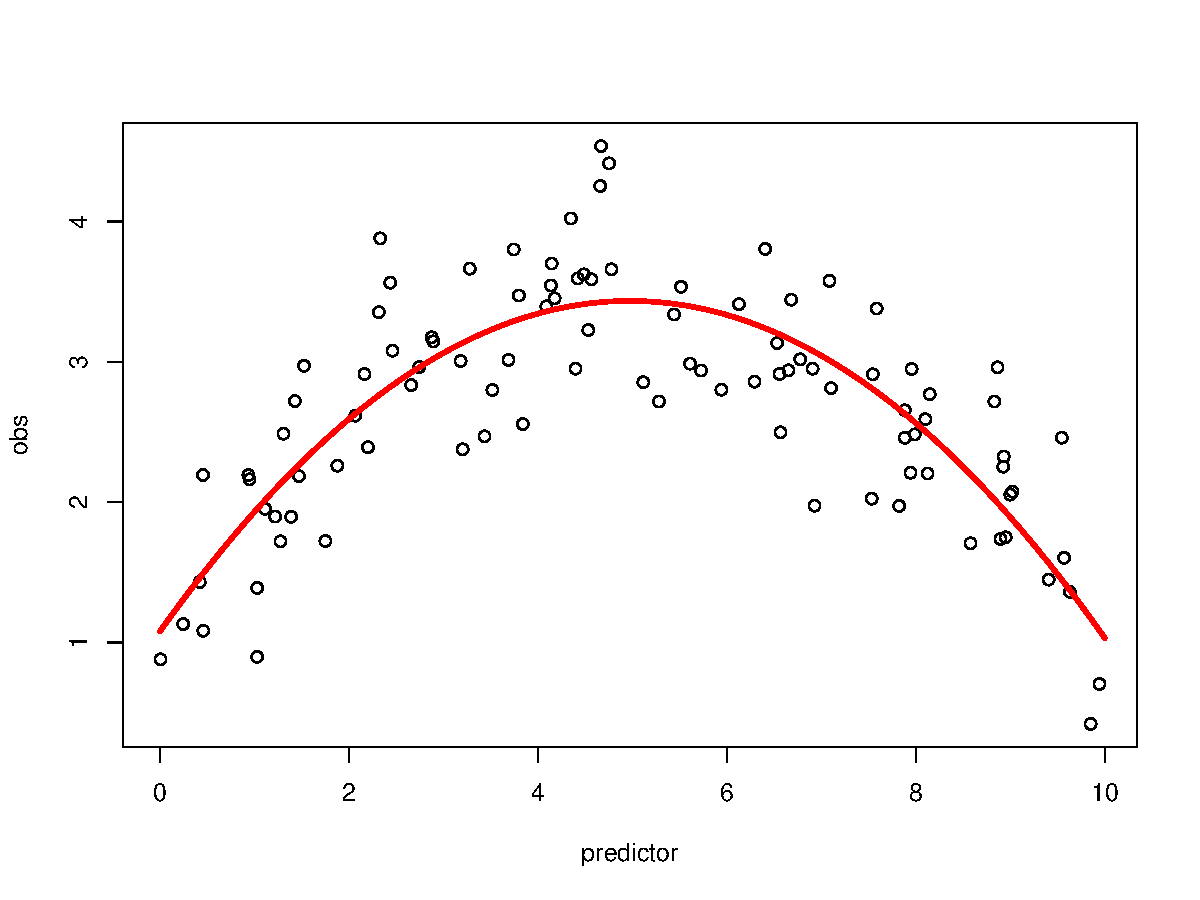
\includegraphics[width=0.8\textwidth,height=0.6\textwidth]{figure/unnamed-chunk-14-1} 

\end{knitrout}
\end{frame}
%%%%%%%%%%%
%%%%%%%%%%%%%%%%%%%%%%%%%%%%%%%%%%%%%%%%%%%%%%%%%%%%%%%%

\begin{frame}
  \begin{center}
    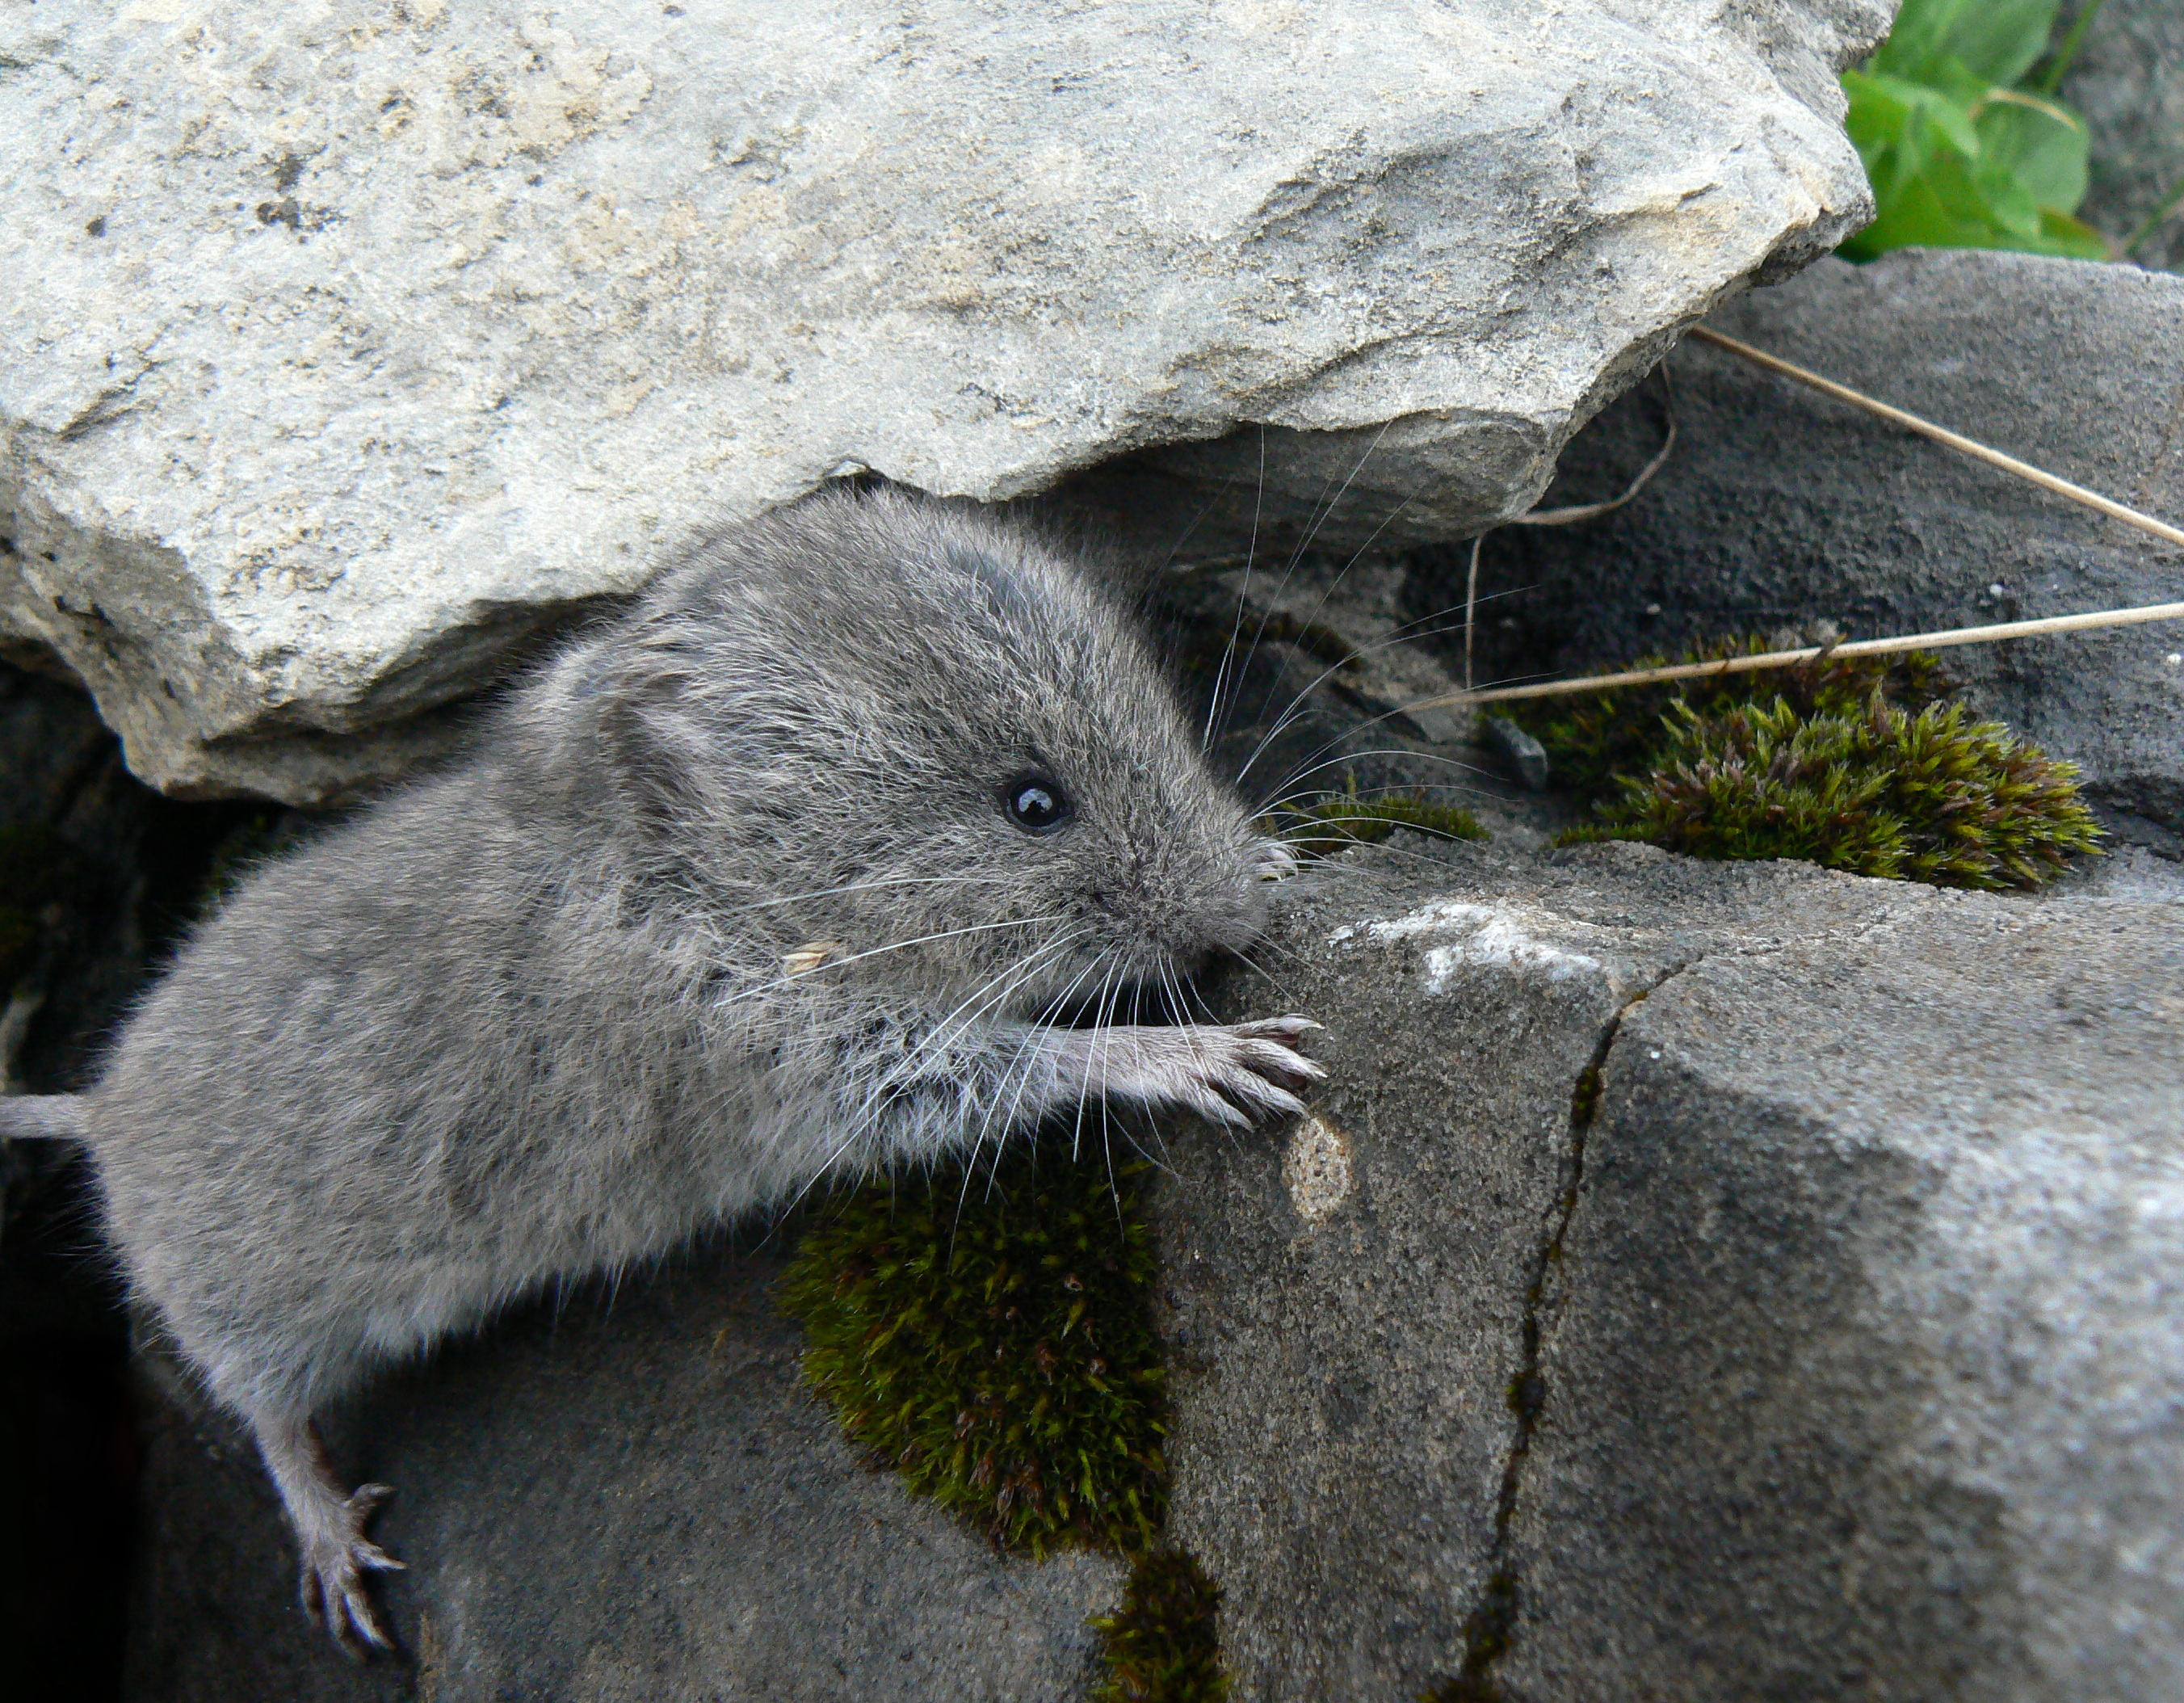
\includegraphics[width=0.5\textwidth]{Figures/brain.jpg}
  \end{center}
\end{frame}

\section{A puzzling but simple problem: Over-fit and collinearity}

\begin{frame}[fragile]{Over-fit and collinearity}
\begin{alertblock}{Small exercise}
Load Cdata.csv, fit models of y predited by x1 and x2, or x2 and x3.\\ Something is weird, what is going on? What to do?
\end{alertblock}





\end{frame}
%%%%%%%%%%%

\section{Heteroschedasticity: the spooky word}

\begin{frame}[fragile]{Exponential data}



Load the dataset \texttt{htrsdt.csv}.

\begin{knitrout}\small
\definecolor{shadecolor}{rgb}{0.843, 0.867, 0.922}\color{fgcolor}\begin{kframe}
\begin{alltt}
\hlkwd{plot}\hlstd{(htrsdt}\hlopt{$}\hlstd{x, htrsdt}\hlopt{$}\hlstd{obs,} \hlkwc{ylim} \hlstd{=} \hlkwd{c}\hlstd{(}\hlopt{-}\hlnum{20}\hlstd{,} \hlkwd{max}\hlstd{(obs)))}
\hlkwd{abline}\hlstd{(}\hlkwd{lm}\hlstd{(obs} \hlopt{~} \hlstd{x,} \hlkwc{data}\hlstd{=htrsdt))}
\hlkwd{summary}\hlstd{(}\hlkwd{lm}\hlstd{(obs} \hlopt{~} \hlstd{x,} \hlkwc{data}\hlstd{=htrsdt))}
\hlkwd{plot}\hlstd{(}\hlkwd{lm}\hlstd{(obs} \hlopt{~} \hlstd{x,} \hlkwc{data}\hlstd{=htrsdt))}
\end{alltt}
\end{kframe}
\end{knitrout}
\end{frame}
%%%%%%%%%%%


\begin{frame}[fragile]{Exponential data: prediction}

Make a prediction over the range of x, with prediction interval
\pause
"By-hand"
\begin{knitrout}\small
\definecolor{shadecolor}{rgb}{0.843, 0.867, 0.922}\color{fgcolor}\begin{kframe}
\begin{alltt}
\hlstd{lmhtrsdt} \hlkwb{<-} \hlkwd{lm}\hlstd{(obs} \hlopt{~} \hlstd{x,} \hlkwc{data}\hlstd{=htrsdt)}
\hlstd{x} \hlkwb{<-} \hlkwd{seq}\hlstd{(}\hlkwc{from}\hlstd{=}\hlkwd{min}\hlstd{(x),} \hlkwc{to}\hlstd{=}\hlkwd{max}\hlstd{(x),} \hlkwc{length.out} \hlstd{=} \hlnum{100}\hlstd{)}
\hlstd{predhtrsdt} \hlkwb{<-} \hlkwd{coef}\hlstd{(lmhtrsdt)[}\hlnum{1}\hlstd{]} \hlopt{+} \hlstd{x} \hlopt{*} \hlkwd{coef}\hlstd{(lmhtrsdt)[}\hlnum{2}\hlstd{]}
\end{alltt}
\end{kframe}
\end{knitrout}

\pause
Function predict
\begin{knitrout}\small
\definecolor{shadecolor}{rgb}{0.843, 0.867, 0.922}\color{fgcolor}\begin{kframe}
\begin{alltt}
\hlstd{Xnewdata} \hlkwb{<-} \hlkwd{data.frame}\hlstd{(}\hlkwc{x}\hlstd{=}\hlkwd{seq}\hlstd{(}\hlkwc{from}\hlstd{=}\hlkwd{min}\hlstd{(x),} \hlkwc{to}\hlstd{=}\hlkwd{max}\hlstd{(x),}
                             \hlkwc{length.out} \hlstd{=} \hlnum{100}\hlstd{))}
\hlstd{Xpred} \hlkwb{<-} \hlkwd{predict}\hlstd{(}\hlkwc{object} \hlstd{=}  \hlkwd{lm}\hlstd{(obs} \hlopt{~} \hlstd{x,} \hlkwc{data}\hlstd{=htrsdt),} \hlkwc{newdata} \hlstd{= Xnewdata,}
                 \hlkwc{se.fit} \hlstd{=} \hlnum{TRUE}\hlstd{,} \hlkwc{interval} \hlstd{=} \hlstr{"prediction"}\hlstd{)}
\end{alltt}
\end{kframe}
\end{knitrout}
\pause
\begin{knitrout}\small
\definecolor{shadecolor}{rgb}{0.843, 0.867, 0.922}\color{fgcolor}\begin{kframe}
\begin{alltt}
\hlstd{Xnewdata} \hlkwb{<-} \hlkwd{cbind}\hlstd{(Xnewdata, Xpred)}
\end{alltt}
\end{kframe}
\end{knitrout}

\begin{knitrout}\small
\definecolor{shadecolor}{rgb}{0.843, 0.867, 0.922}\color{fgcolor}\begin{kframe}
\begin{alltt}
\hlkwd{head}\hlstd{(Xnewdata)}
\end{alltt}
\end{kframe}
\end{knitrout}

\end{frame}
%%%%%%%%%%%

\begin{frame}[fragile]{Exponential data: prediction}

\begin{knitrout}\small
\definecolor{shadecolor}{rgb}{0.843, 0.867, 0.922}\color{fgcolor}\begin{kframe}
\begin{alltt}
\hlkwd{plot}\hlstd{(x, obs,} \hlkwc{ylim} \hlstd{=} \hlkwd{c}\hlstd{(}\hlopt{-}\hlnum{100}\hlstd{,} \hlkwd{max}\hlstd{(obs)))}
\hlkwd{lines}\hlstd{(Xnewdata}\hlopt{$}\hlstd{x, Xnewdata}\hlopt{$}\hlstd{fit.fit,} \hlkwc{col}\hlstd{=}\hlstr{"red"}\hlstd{,} \hlkwc{lwd}\hlstd{=}\hlnum{3}\hlstd{)}
\hlkwd{lines}\hlstd{(Xnewdata}\hlopt{$}\hlstd{x, Xnewdata}\hlopt{$}\hlstd{fit.lwr,} \hlkwc{col}\hlstd{=}\hlstr{"red"}\hlstd{,} \hlkwc{lty}\hlstd{=}\hlnum{2}\hlstd{,} \hlkwc{lwd}\hlstd{=}\hlnum{3}\hlstd{)}
\hlkwd{lines}\hlstd{(Xnewdata}\hlopt{$}\hlstd{x, Xnewdata}\hlopt{$}\hlstd{fit.upr,} \hlkwc{col}\hlstd{=}\hlstr{"red"}\hlstd{,} \hlkwc{lty}\hlstd{=}\hlnum{2}\hlstd{,} \hlkwc{lwd}\hlstd{=}\hlnum{3}\hlstd{)}
\end{alltt}
\end{kframe}
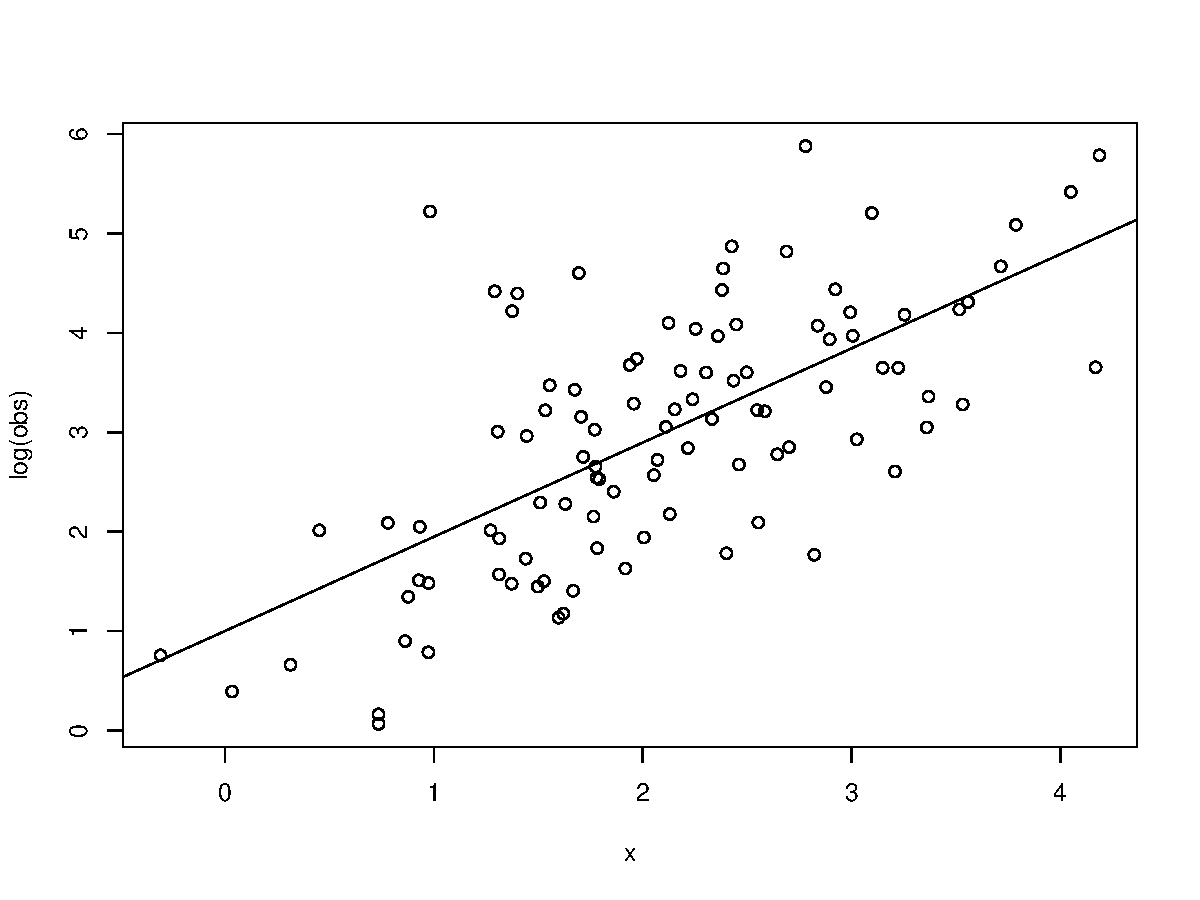
\includegraphics[width=0.8\textwidth,height=0.6\textheight]{figure/unnamed-chunk-23-1} 

\end{knitrout}

\end{frame}
%%%%%%%%%%%
%
\begin{frame}[fragile]{Exponential data: confidence}

\textbf{Prediction interval:} Where the model predicts new data would be sampled, including variation unrelated to predictor\\
\pause
\textbf{Confidence interval:} Where your model predicts the MEAN new data would be sampled; or where is the true relationship with predictor
\begin{knitrout}\small
\definecolor{shadecolor}{rgb}{0.843, 0.867, 0.922}\color{fgcolor}\begin{kframe}
\begin{alltt}
\hlstd{Xconf} \hlkwb{<-} \hlkwd{predict}\hlstd{(}\hlkwc{object} \hlstd{=} \hlkwd{lm}\hlstd{(obs} \hlopt{~} \hlstd{x),} \hlkwc{newdata} \hlstd{= Xnewdata,}
                 \hlkwc{se.fit} \hlstd{=} \hlnum{TRUE}\hlstd{,} \hlkwc{interval} \hlstd{=} \hlstr{"confidence"}\hlstd{)}
\hlstd{Xnewdata[,}\hlkwd{c}\hlstd{(}\hlstr{"conf.lwr"}\hlstd{,} \hlstr{"conf.upr"}\hlstd{)]} \hlkwb{<-}  \hlstd{Xconf}\hlopt{$}\hlstd{fit[,}\hlnum{2}\hlopt{:}\hlnum{3}\hlstd{]}
\end{alltt}
\end{kframe}
\end{knitrout}


\end{frame}
%%%%%%%%%%%
\begin{frame}[fragile]{Exponential data: confidence}

\begin{knitrout}\small
\definecolor{shadecolor}{rgb}{0.843, 0.867, 0.922}\color{fgcolor}\begin{kframe}
\begin{alltt}
\hlkwd{plot}\hlstd{(x, obs,} \hlkwc{ylim} \hlstd{=} \hlkwd{c}\hlstd{(}\hlopt{-}\hlnum{100}\hlstd{,} \hlkwd{max}\hlstd{(obs)))}
\hlkwd{lines}\hlstd{(Xnewdata}\hlopt{$}\hlstd{x, Xnewdata}\hlopt{$}\hlstd{fit.fit,} \hlkwc{col}\hlstd{=}\hlstr{"red"}\hlstd{,} \hlkwc{lwd}\hlstd{=}\hlnum{3}\hlstd{)}
\hlkwd{lines}\hlstd{(Xnewdata}\hlopt{$}\hlstd{x, Xnewdata}\hlopt{$}\hlstd{fit.lwr,} \hlkwc{col}\hlstd{=}\hlstr{"red"}\hlstd{,} \hlkwc{lty}\hlstd{=}\hlnum{2}\hlstd{,} \hlkwc{lwd}\hlstd{=}\hlnum{3}\hlstd{)}
\hlkwd{lines}\hlstd{(Xnewdata}\hlopt{$}\hlstd{x, Xnewdata}\hlopt{$}\hlstd{fit.upr,} \hlkwc{col}\hlstd{=}\hlstr{"red"}\hlstd{,} \hlkwc{lty}\hlstd{=}\hlnum{2}\hlstd{,} \hlkwc{lwd}\hlstd{=}\hlnum{3}\hlstd{)}
\hlkwd{lines}\hlstd{(Xnewdata}\hlopt{$}\hlstd{x, Xnewdata}\hlopt{$}\hlstd{conf.lwr,} \hlkwc{col}\hlstd{=}\hlstr{"blue"}\hlstd{,} \hlkwc{lty}\hlstd{=}\hlnum{2}\hlstd{,} \hlkwc{lwd}\hlstd{=}\hlnum{3}\hlstd{)}
\hlkwd{lines}\hlstd{(Xnewdata}\hlopt{$}\hlstd{x, Xnewdata}\hlopt{$}\hlstd{conf.upr,} \hlkwc{col}\hlstd{=}\hlstr{"blue"}\hlstd{,} \hlkwc{lty}\hlstd{=}\hlnum{2}\hlstd{,} \hlkwc{lwd}\hlstd{=}\hlnum{3}\hlstd{)}
\end{alltt}
\end{kframe}
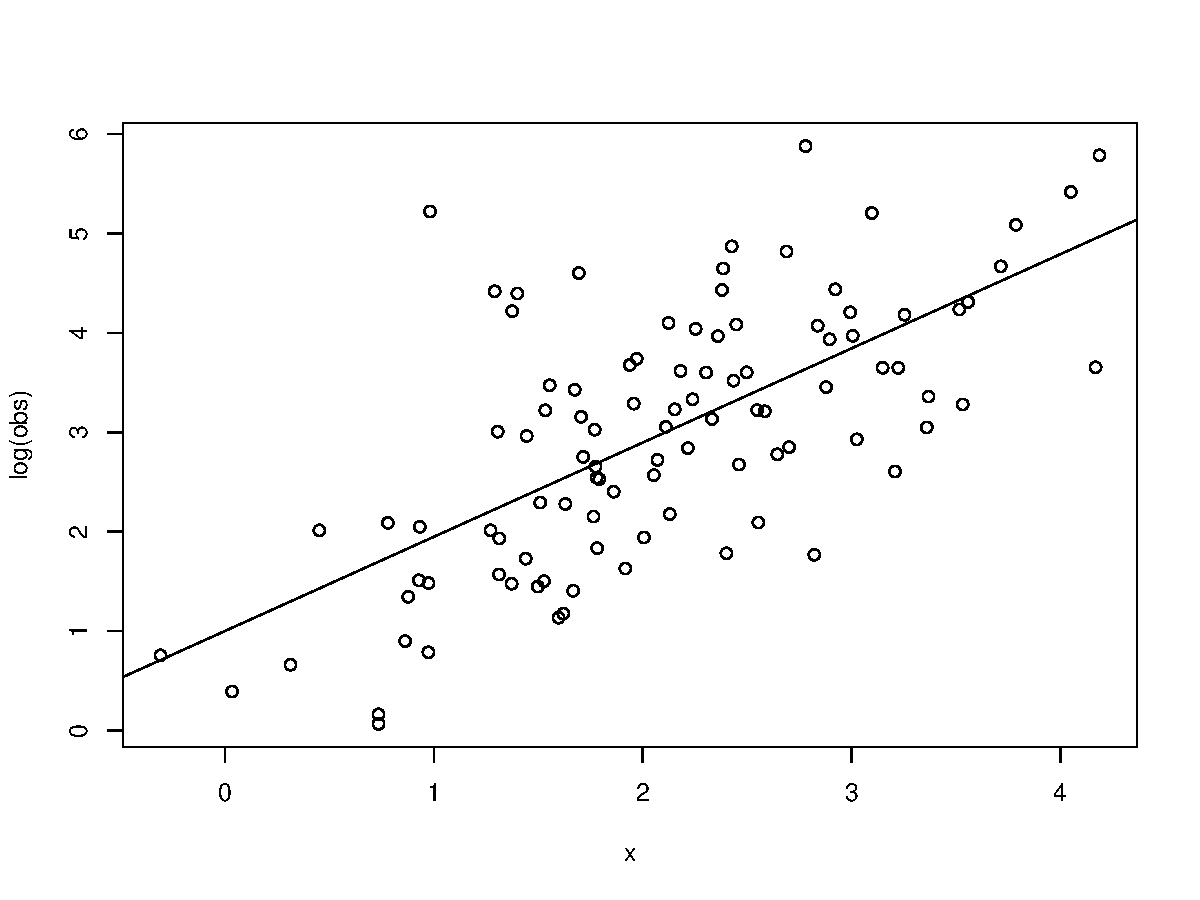
\includegraphics[width=0.8\textwidth,height=0.6\textheight]{figure/unnamed-chunk-25-1} 

\end{knitrout}

\end{frame}
%%%%%%%%%%
%
\begin{frame}[fragile]{Exponential data: fix}
\begin{block}{Model sufficient to show positive relationship\dots BUT}
  \begin{itemize}
    \item no negative values should exist
    \item too many outliers
    \item too much uncertainty on the left\dots
  \end{itemize}
\end{block}

\begin{block}{Consequences:}
\begin{itemize}
\item impossible to understand the biological mechanism
\item impossible to predict future observations
\end{itemize}
\end{block}

What to do?
\end{frame}
%%%%%%%%%%M

\begin{frame}[fragile]{Exponential data: fix}

Log-transform
\begin{knitrout}\small
\definecolor{shadecolor}{rgb}{0.843, 0.867, 0.922}\color{fgcolor}\begin{kframe}
\begin{alltt}
\hlkwd{plot}\hlstd{(x,} \hlkwd{log}\hlstd{(obs));} \hlkwd{abline}\hlstd{(}\hlkwd{lm}\hlstd{(}\hlkwd{log}\hlstd{(obs)} \hlopt{~} \hlstd{x))}
\hlkwd{summary}\hlstd{(}\hlkwd{lm}\hlstd{(}\hlkwd{log}\hlstd{(obs)} \hlopt{~} \hlstd{x))}
\hlkwd{plot}\hlstd{(}\hlkwd{lm}\hlstd{(}\hlkwd{log}\hlstd{(obs)} \hlopt{~} \hlstd{x))}
\end{alltt}
\end{kframe}
\end{knitrout}

\pause
By the way, the simulation process:
\begin{knitrout}\small
\definecolor{shadecolor}{rgb}{0.843, 0.867, 0.922}\color{fgcolor}\begin{kframe}
\begin{alltt}
\hlkwd{set.seed}\hlstd{(}\hlnum{123}\hlstd{)}
\hlstd{x} \hlkwb{<-} \hlnum{2}\hlopt{+}\hlkwd{rnorm}\hlstd{(}\hlnum{100}\hlstd{)}
\hlstd{y} \hlkwb{<-} \hlnum{1} \hlopt{+} \hlstd{x} \hlopt{+} \hlkwd{rnorm}\hlstd{(}\hlnum{100}\hlstd{)}
\hlstd{obs} \hlkwb{<-} \hlkwd{exp}\hlstd{(y)}
\end{alltt}
\end{kframe}
\end{knitrout}

\end{frame}
%%%%%%%%%%M

\begin{frame}[fragile]{Exponential data: other fix}
Non-parametric statistics:\\ 
Rank observations, do greater ranks go together?\\ \pause
Case of two continuous variable: Spearman's rank correlation
\pause
\begin{knitrout}\small
\definecolor{shadecolor}{rgb}{0.843, 0.867, 0.922}\color{fgcolor}\begin{kframe}
\begin{alltt}
\hlkwd{cor.test}\hlstd{(}\hlkwc{x} \hlstd{= x,} \hlkwc{y} \hlstd{= obs,} \hlkwc{method} \hlstd{=} \hlstr{"spearman"}\hlstd{)}
\end{alltt}
\begin{verbatim}

	Spearman's rank correlation rho

data:  x and obs
S = 60622, p-value < 2.2e-16
alternative hypothesis: true rho is not equal to 0
sample estimates:
      rho 
0.6362316 
\end{verbatim}
\end{kframe}
\end{knitrout}
\pause
Significant positive correlation confirmed, BUT, no biological mechanism, little predictive power.

\end{frame}
%%%%%%%%%%%

\begin{frame}[fragile]{Practice lm() with parasites}


  
  \begin{alertblock}{What explains variation in parasitic load?}
  You collected ecto-parasites on some furry large mammals at three locations. Parasites break easily when we collect them and are impossible to count, so we decide to measure parasitic load as their mass. \textbf{Why do some mammals have larger parasitic load?} \pause
    \begin{itemize}
      \item Load the \texttt{Para.csv} data (don't forget: str(), summary(), plot()\dots)
      \item Model \verb+Parasite_Mass+ using \texttt{lm()}
      \item Find what variables predict \verb+Parasite_Mass+
      \item How good are your models? Assumptions? Prediction?
      \item What biological interpretation can you imagine?
      \end{itemize}
  \end{alertblock}
  
\end{frame}
%%%%%%%%%%%


%%%%%%%%%%%%%%%%%%%%%%%%%%%%%%%%%%%%%%%%%%%%%%%%%%%%%%%%%%%%%%%%%%%%
%%%%%%%%%%%%%%%%%%%%%%%%%%%%%%%%%%%%%%%%%%%%%%%%%%%%%%%%%%%%%%%%%%%%


%%%%%%%%%%%%%%%%%%%%%%%%%%%%%%%%%%%%%%%%%%%%%%%%%%%%%%%%%%%%%%%%%%%%%%%%%%%%%%%%%%%%%%%%
%%%%%%%%%%%%%%%%%%%%%%%%%%%%%%%%%%%%%%%%%%%%%%%%%%%%%%%%%%%%%%%%%%%%%%%%%%%%%%%%%%%%%%%%
\begin{frame}{Linear model basic assumptions}
Not necessarily wrong, but typical interpretation assumes:
 \begin{block}{}
     \begin{itemize}
      \item Linear combination of parameters (including transformation, polynoms, interactions\dots)
      \item Predictor not perfectly correlated 
       \item {\color{red!20!black}{Measurement error in predictors}}
       \item {\color{red!50!black}{Gaussian error distribution}}
       \item {\color{red!70!black}{Homoscedasticity (constant error variance)}}
       \item {\color{red!99!black}{Independence of error}}
     \end{itemize}
 \end{block}
 
 \pause
 \begin{exampleblock}{TEASER: The most difficult problems are the reason for}
  \begin{itemize}[<+->]
    \item Multiple regression
    \item Generalized Linear Models
    \item (Generalized) Linear Mixed Models
    \item Non-linear models
  \end{itemize}
 \end{exampleblock}
\end{frame}
%%%%%%%%%%%

\section{If time permits: multiple regression}

\begin{frame}{Improvisation}

\end{frame}
%%%%%%%%%%%
%%%%%%%%%%%%%%%%%%%%%%%%%%%%%%%%%%%%%%%%%%%%%%%%%%%%%%%%%%%%%%%%%%%%%%%%%%%%%%%%%
%%%%%%%%%%%%%%%%%%%%%%%%%%%%%%%%%%%%%%%%%%%%%%%%%%%%%%%%%%%%%%%%%%%%%%%%%%%%%%%%%
% 
% \section*{Feedback wanted!}
% 
% \begin{frame}{What do you want to learn about?}
% 
% \begin{alertblock}{Topics}
%   \begin{itemize}
%     \item 
%   \end{itemize}
% \end{alertblock}
% 
% \end{frame}
% %%%%%%%%%%%


\end{document}
